%%%%%%%%%%%%%%%%%%%%%%%%%%%%%%%%%%%%%%%%%%%%%%%%%%%%%%%%%%%%%%%%%%%%%%%%%%%%%%%%
%%%%%%%%%%%%%%%%%%%%%%%%%%%%%%%%%%%%%%%%%%%%%%%%%%%%%%%%%%%%%%%%%%%%%%%%%%%%%%%%
%%                                                                            %%
%% opintnaytepohja.tex versio 3.20 (2018/08/31)                               %%
%% Opinnäytepohja käytettäväksi aaltothesis.sty (versio 3.20) -tyylitiedoston %%
%% kanssa.                                                                    %%
%% Toimiakseen paketti tarvitsee pdfx.sty v. 1.5.84 (2017/05/18) tai uudempi. %%
%% The LaTeX template file to be used with the aaltothesis.sty (version 3.20) %%
%% style file.                                                                %%
%% This package requires pdfx.sty v. 1.5.84 (2017/05/18) or newer.            %%
%%                                                                            %%
%% This is licensed under the terms of the MIT license below.                 %%
%%                                                                            %%
%% Written by Luis R.J. Costa.                                                %%
%% Currently developed at the Learning Services of Aalto University School of %%
%% Electrical Engineering by Luis R.J. Costa since May 2017.                  %%
%%                                                                            %%
%% Copyright 2017-2018, by Luis R.J. Costa, luis.costa@aalto.fi,              %%
%% Copyright 2017-2018 Swedish translations in aaltothesis.cls by Elisabeth   %%
%% Nyberg, elisabeth.nyberg@aalto.fi and Henrik Wallén,                       %%
%% henrik.wallen@aalto.fi.                                                    %%
%% Copyright 2017-2018 Finnish documentation in the template opinnatepohja.tex%%
%% by Perttu Puska, perttu.puska@aalto.fi, and Luis R.J. Costa.               %%
%% Copyright 2018 English template thesistemplate.tex by Luis R.J. Costa.     %%
%% Copyright 2018 Swedish template kandidatarbetsbotten.tex by Henrik Wallen. %%
%%                                                                            %%
%% Permission is hereby granted, free of charge, to any person obtaining a    %%
%% copy of this software and associated documentation files (the "Software"), %%
%% to deal in the Software without restriction, including without limitation  %%
%% the rights to use, copy, modify, merge, publish, distribute, sublicense,   %%
%% and/or sell copies of the Software, and to permit persons to whom the      %%
%% Software is furnished to do so, subject to the following conditions:       %%
%% The above copyright notice and this permission notice shall be included in %%
%% all copies or substantial portions of the Software.                        %%
%% THE SOFTWARE IS PROVIDED "AS IS", WITHOUT WARRANTY OF ANY KIND, EXPRESS OR %%
%% IMPLIED, INCLUDING BUT NOT LIMITED TO THE WARRANTIES OF MERCHANTABILITY,   %%
%% FITNESS FOR A PARTICULAR PURPOSE AND NONINFRINGEMENT. IN NO EVENT SHALL    %%
%% THE AUTHORS OR COPYRIGHT HOLDERS BE LIABLE FOR ANY CLAIM, DAMAGES OR OTHER %%
%% LIABILITY, WHETHER IN AN ACTION OF CONTRACT, TORT OR OTHERWISE, ARISING    %%
%% FROM, OUT OF OR IN CONNECTION WITH THE SOFTWARE OR THE USE OR OTHER        %%
%% DEALINGS IN THE SOFTWARE.                                                  %%
%%                                                                            %%
%%                                                                            %%
%%%%%%%%%%%%%%%%%%%%%%%%%%%%%%%%%%%%%%%%%%%%%%%%%%%%%%%%%%%%%%%%%%%%%%%%%%%%%%%%
%%                                                                            %%
%%                                                                            %%
%% Esimerkki opinnäytteen tekemisestä LaTeX:lla                               %%
%% Alkuperäinen versio ja nykinen kehitystyö Luis Costa, muutokset            %%
%% suomenkieliseen tekstipohjaan Perttu Puska.                                %%
%% Ruotsinkielen tuki lisätty 15092014                                        %%
%% PDF/A-1b -tuki lisätty 15092017                                            %%
%% PDF/A-2b -tuki lisätty 24042018                                            %%
%%                                                                            %%
%% Tähän esimerkkiin kuuluu tiedostot                                         %%
%%        opinnaytepohja.tex (versio 3.20) (suomenkielinen pohja)             %%
%%        thesistemplate.tex (versio 3.20) (for text in English)              %%
%%        kandidatarbetsbotten.tex (versio 1.00) (ruotsinkielinen kandipohja) %%
%%        aaltothesis.cls (versio 3.20)                                       %%
%%        linediagram.eps                                                     %%
%%        curves.eps                                                          %%
%%        linediagram.pdf                                                     %%
%%        curves.pdf                                                          %%
%%        ledspole.jpg                                                        %%
%%                                                                            %%
%%                                                                            %%
%% Kääntäminen Linuxissa joko                                                 %%
%% pdflatex: (suositeltava tapa)                                              %%
%%             $ pdflatex opinnaytepohja                                      %%
%%             $ pdflatex opinnaytepohja                                      %%
%%                                                                            %%
%%   Tuloksena on tiedosto opinnaytepohja.pdf, joka on PDF/A-standardin       %%
%%   mukainen, jos olet valinnut oikeat \documentclass -optiot (kts. alla) ja %%
%%   ja käyttämäsi kuvatiedostoissa ei ole ongelmia.                          %%
%%                                                                            %%
%% Tai                                                                        %%
%% latex: (ei ole suositeltava tapa)                                          %%
%%             $ latex opinnaytepohja                                         %%
%%             $ latex opinnaytepohja                                         %%
%%                                                                            %%
%%   Tuloksena on tiedosto opinnayte.dvi, joka muutetaan ps-muotoon           %%
%%   seuraavasti                                                              %%
%%                                                                            %%
%%             $ dvips opinnaytepohja -o                                      %%
%%                                                                            %%
%%   ja edelleen pdf-muotoon seuraavasti                                      %%
%%                                                                            %%
%%             $ ps2pdf opinnaytepohja.ps                                     %%
%%                                                                            %%
%%   Tämä pdf EI ole pdf/a -tiedosto vaan se pitää muuttaa sellaiseksi esim.  %%
%%   Acrobat Pro- tai PDF-XChange -ohjelmalla.                                %%
%%                                                                            %%
%%                                                                            %%
%% Selittävät kommentit on tässä esimerkissä varustettu %%-merkeillä ja       %%
%% muutokset, joita käyttäjä voi tehdä, on varustettu %-merkeillä             %%
%%                                                                            %%
%%%%%%%%%%%%%%%%%%%%%%%%%%%%%%%%%%%%%%%%%%%%%%%%%%%%%%%%%%%%%%%%%%%%%%%%%%%%%%%%
%%%%%%%%%%%%%%%%%%%%%%%%%%%%%%%%%%%%%%%%%%%%%%%%%%%%%%%%%%%%%%%%%%%%%%%%%%%%%%%%
%%
%% MIKÄ on PDF/A?
%%
%% PDF/A on ISO-standardoitu versio pdf-tiedostosta. Standardin tavoite on, että
%% tiedosto on toistettavissa myös pitkänkin ajan kuluessa. PDF/A eroaa pdf:stä
%% siinä, että se sallii vain sellaisia pdf-ominaisuuksia, jotka tukevat
%% tiedoston pitkäaikaista arkistointia. Esim. PDF/A vaati, että kaikki käytetyt
%% fontit ovat mukana tiedostossa, mutta tavallisessa pdf:ssä voi olla niin,
%% että tiedostossa on vain linkki tiedostonlukijan tietokonejärjestelmän
%% fontteihin. PDF/A vaatii myös tietoa mm. värimäärittelystä ja käytetystä
%% salauksesta.
%% Tällä hetkellä PDF/A standardeja on kolme:
%% PDF/A-1: perustana PDF 1.4, standardi ISO19005-1, julkaistu vuonna 2005.
%%          Kaikki perusvaatimukset pitkäaikaiseen arkistointiin käytössä.
%% PDF/A-2: perustana PDF 1.7, standardi ISO19005-2, julkaistu vuonna 2011.
%%          Yllä olevan lisäksi tukee mm. OpenType-fonttien sisällyttämistä,
%%          läpinäkyvyyttä värimäärittelyssä ja digitaalisia allekirjoituksia.
%% PDF/A-3: perustana PDF 1.7, standardi ISO19005-3, julkaistu vuonna 2012.
%%          Eroaa edellisestä ainoastaan siinä, että se sallii missä tahansa
%%          tiedostoformaatissa (esim. xml, csv, cad, taulukkolaskentaformaatit,
%%          tekstinkäsittelyformaatit) olevien tiedostojen sisällyttämisen.
%% PDF/A-1 tiedostot eivät välttämättä ole PDF/A-2 -yhteensopivia eikä PDF/A-2
%% tiedostot ole PDF/A-1 -yhteensopivia.
%% Kaikista yllä olevista PDF/A-standardeista on kaksi tasoa:
%% b: (basic) vaatii, että tiedoston visuaalinen ilme on luotettavasti
%%    toistettavissa.
%% a: (accessible) b-tason vaatimuksien lisäksi, määrittelee kuinka saavutettava
%%    pdf-tiedosto on mm. vammaisteknologiaa hyödynttävissä ohjelmistoissa
%%    (esim. kosketusruutua käytettävissä laitteissa).
%% Lisätietoa PDF/A:sta esim. https://en.wikipedia.org/wiki/PDF/A tai
%%
%%
%% MINKÄ PDF/A -standardin mukaan teen opinnäytetyöni?
%%
%% Ensisijaisesti PDF/A-1b -standardin mukaan. Kuvaajat ja kuvat mitä
%% tyypillisesti käytetään opinnäytetyössä eivät tarvitse
%% läpinäkyvyysominaisuuksia. Perus '2D' -näkymä on riittävä. Opinnäytetyössä
%% käytettävät fontit on määritelty tässä pohjassa eikä niitä pidä muuttaa. Jos
%% käytät kuvia, jossa läpikäkyvyysominaisuuksillä on merkitystä, käytä PDF/A-2b
%% -standardia. Älä käytä PDF/A-3b -standardia opinnäytetyössäsi.
%%
%%
%% MITKÄ kuvaformaatteja voin käyttää PDF/A-tiedoston tekemisessä?
%%
%% Kun käytät pdflatexia työsi kääntämisessä suosi pdf-formaattia, mutta voit
%% käytä myös jpg- ja/tai png-formmaatia eteenkin valokuvissa.
%% Pdf-muotoisten kuvien kanssa voi tulla ongelmia PDF/A -yhteesopivuuden
%% kanssa, mm. jos fontit eivät ole upotettu tiedostoon.
%% Älä käytä PDF/A-formaattia kuvatiedostoissa.
%% Jos kuitenkin käytät perus latexia työsi kääntämisessä, ainoa sallittu
%% kuvaformaatti on eps. ÄLÄ käytä ps-formaattia kuvissasi.
%%
%% KÄYTÄ näistä yhtä:
%% * ensimmäinen, jos käytät pdflatexia, joka kääntää tekstin suoraan
%%   pdf/a-tiedostoksi ja haluat julkaista opinnäytetyösi verkossa
%% * toinen, jos haluat tulostaa opinnäytteesi kansitettavaksi
%% * kolmas jos haluat tuottaa ps-tiedostoa ja siitä pdf/a:ta

\documentclass[finnish, 12pt, a4paper, elec, utf8, a-1b, online]{aaltothesis}
%\documentclass[finnish, 12pt, a4paper, elec, utf8, a-1b]{aaltothesis}
%\documentclass[finnish, 12pt, a4paper, elec, dvips, online]{aaltothesis}

%% Kirjoita y.o. \documentclass optioiksi
%% * korkeakoulusi näistä: arts, biz, chem, elec, eng, sci
%% * editorisi käyttämä merkkikoodaustapa: utf8, latin1
%% * opinnäytetyön kieli: finnish, english, swedish
%% * tee arkistointikelpoista PDF/A-1b tai PDF/A-2b pdf-tiedosto: a-1b, a-2b
%%                         (pdflatex tuottaa tavallisen metadataa sisältävän
%%                          pdf-tiedoston ilman a-*b optiota)
%% * verkkoon menevä symmetrinen taitto, sinisellä hypertekstillä: online
%%                         (oletusarvo on leveä marginaali sivun sidonta
%%                          puolella ja musta hyperteksti)
%% * kaksipuolinen tulostus: twoside (oletusarvo on yksipuolinen tulostus)
%%
%% Käytä yhtä näistä, jos kirjoitat englanniksi. Katso englanninokset
%% tiedostosta thesistemplate.tex.
%\documentclass[english, 12pt, a4paper, elec, utf8, a-1b, online]{aaltothesis}
%\documentclass[english, 12pt, a4paper, elec, utf8, a-1b]{aaltothesis}
%\documentclass[english, 12pt, a4paper, elec, dvips, online]{aaltothesis}
%%
%% Jos kirjoitat ruotsiksi, katso kandidatarbetsbotten.tex ruotsinskielistä
%% kandipohjaa.
%\documentclass[swedish, 12pt, a4paper, elec, utf8, a-1b, online]{aaltothesis}
%\documentclass[swedish, 12pt, a4paper, elec, utf8, a-1b]{aaltothesis}
%\documentclass[swedish, 12pt, a4paper, elec, dvips, online]{aaltothesis}


\usepackage{graphicx}

% Matematiikan fontteja, symboleja ja muotoiluja lisää, näitä tarvitaan usein
\usepackage{amsfonts, amssymb, amsbsy, amsmath}

\usepackage{setspace}
\onehalfspacing

% Tutkinto-ohjelma
\degreeprogram{Elektroniikka ja sähkötekniikka}

% Pääaine
\major{Elektroniikka ja sähkötekniikka}

% Pääainekoodi
\code{ELEC3013}

% Tutkinnon taso
\univdegree{BSc}

% Oma nimi
\thesisauthor{Toni Ojala}

% Opinnäytetyön otsikko
\thesistitle{Adaptiivinen videokuva eri verkkoselaimilla}

% Paikka
\place{Espoo}

% Kandidaatintyön päivämäärä on sen esityspäivämäärä
\date{8.9.2022}

% Kandidaattiseminaarin vastuuopettaja
\supervisor{Yliopistonlehtori Markus Turunen}

% Kandidaatintyön ohjaaja(t) tai diplomityön ohjaaja(t). Ohjaajia saa olla korkeintaan kaksi.
\advisor{DI Juha Järvinen}

% Aaltologo
% Syntaksi:
% \uselogo{aaltoRed|aaltoBlue|aaltoYellow|aaltoGray|aaltoGrayScale}{?|!|''}
% Logon kieli on sama kuin dokumentin kieli
\uselogo{aaltoBlack}{!}

% Suomenkielinen tiivistelmä:
% Kaikki tiivistelmässä tarvittava tieto (nimesi, työnnimi, jne.) käytetään
% niin kuin se on yllä määritelty.
% Tiivistelmän avainsanat:
% Huom! Avainsanat erotetaan toisistaan \spc -makrolla
\keywords{
  verkkoselain\spc
  adaptiivinen videokuva\spc
  suoratoisto
}

% Tiivistelmän tekstiosa
% Tämä teksti sisältyy pdf-tiedoston metadataa ja tulee myös tiivistelmälomakkeeseen.
\thesisabstract{
  Tässä työssä on tutkittu kirjallisuuskatsauksena viittä suosituinta verkkoselainta (Google Chrome, Mozilla Firefox, Apple Safari, Microsoft Edge ja Opera) adaptiivisen videokuvan näkökulmasta. Kyseiset selaimet käyttävät vain kolmea eri selainmoottoria ja ovat ominaisuuksiltaan hyvin samankaltaisia. \\\\ Verkkokäytössä olevat videoformaatit rajoittuvat olennaisesti kahteen: MP4 ja WebM. Molemmat formaatit sopivat erinomaisesti verkkokäyttöön hyvän pakkaussuhteen takia. Eroja löytyy lähinnä koodekkituen osalta. \\\\ Lähes kaikki internetin adaptiivinen videokuva toimitetaan HTTP:n avulla joko DASH:llä tai HLS:llä. Nuo kaksi siirtoprotokollaa ovat lähes identtisiä toimintaperiaatteeltaan. Isoin ero on se, että DASH on standardoitu ja että HLS on laajemmin tuettu. \\\\ Työn tärkeimmät tulokset on kiteytettävissä siihen, että selainten välillä on vain vähän eroja. Isoin ero on siirtoprotokollatuessa sekä koodekkituessa, sillä Safari ei tue DASH:ä siirtoprotokollana, eikä AV1:tä koodekkina, mutta tukee ainoana H.265/HEVC-koodekkia.\\
}

% Tekijänoikeusteksti. Tekijänoikeus on tekijällä riippumatta siitä onko copyright -merkintä näkyvissä vai ei.
% Halutessasi voit jakaa työsi Creative Commons -lisensillä (katso creativecommons.org),
% jolloin lisenssitekstin on oltava näkyvissä. Kirjoita tähän haluamasi tekijänoikeustektin.
% Se kirjautuu myös pdf-tiedoston metadataan.
% Syntaksi:
% \copyrigthtext{metadatateksti}{sivulle näkyviin tuleva teksti}
%
% A.o. metadataan menevässä tekstissä on käytettävä \noexpand -makroa ennen
% \copyright -erikoismerkkiä ja lisäksi makrot (tässä \copyright ja \year) on
% erotettava seuraavasta tekstistä \ -merkillä (välilyöntimerkki).
% \copyrighttext-makron argumentissa olevat makrot automaattisesti hakevat vuosiluvun ja tekijän nimi.
% (Huom! \ThesisAuthor on aaltothesis.cls -tyylitiedoston sisäinen makro).
% Toki saman tekstin olisi voinut kirjoittaa yksinkertaisesti näin:
% \copyrighttext{Copyright \noexpand\copyright\ 2018 Teemu Teekkari}
% {Copyright \copyright{} 2018 Teemu Teekkari}
\copyrighttext{Copyright \noexpand\copyright\ \number\year\ \ThesisAuthor}
{Copyright \copyright{} \number\year{} \ThesisAuthor}


\begin{document}


% Kansilehti
\makecoverpage{}

% Tehdään tekijänoikeusteksti näkyväksi.
% Halutessasi voit jättää tekijänoikeustekstin pois luettavasta pdf
% -tiedostosta. Tämä voi tuntua hyvältä ajatukselta paperille tulostetulla
% versiossa eteenkin, jos sivun ainoa teksti on "Copyright (c) vvvv Teemu
% Teekkari". Suositus on kuitenkin jättää teksti näkyviin.
\makecopyrightpage{}

% Suomenkielinen tiivistelmä
% Kaikki tiivistelmässä tarvittava tieto (nimi, työn nimi jne.) käytetään niin kuin se on yllä määritelty.
\begin{abstractpage}[finnish]
  \abstracttext{}
\end{abstractpage}

% \thesisabstract -makrossa kirjoitettu teksti on tallennettu makroon
% \abstractext, jolloin voit siirtää metadataan menevä teksti sellaisenaan näin:
%\begin{abstractpage}[finnish]
%	\abstracttext{}
%\end{abstractpage}

% Pakotetaan varmuuden vuoksi esipuheen jälkeinen osa alkamaan uudelta sivulta
\newpage

% Sisällysluettelo
\thesistableofcontents

% Symbolit ja lyhenteet
\mysection{Käsitteet ja lyhenteet}

\subsection*{Käsitteet}
\begin{tabular}{ll}
  HTML5           & Yleiskäsite moderneille verkkoteknologioille, joihin kuuluu \\
                  & HTML, CSS ja JavaScript \\
  HTTP            & Protokolla, jota selaimet ja palvelimet käyttävät tiedonsiirtoon. \\
                  & Määrittää miten esim. teksti, kuva ja video siirretään verkossa. \\
  Koodekki        & Laite tai ohjelmisto, joka mahdollistaa esimerkiksi videon \\
                  & pakkaamisen tai purkamisen. \\
  URL             & Jonkin verkkoresurssin (lähtäkohtaisesti verkkosivun) osoite.\\
  Verkkoselain    & Tietokoneohjelma, jota käytetään World Wide Webin \\
                  & tai paikallisen verkkosivun käyttämiseen \\
  World Wide Web  & Internet-verkossa toimiva hajautettu tietojärjestelmä \\
  WorldWideWeb    & Ensimmäinen verkkoselain
\end{tabular}

\subsection*{Lyhenteet}
\begin{tabular}{ll}
  DASH      & Dynamic Adaptive Streaming over HTTP, \\
            & tunnetaan myös nimellä MPEG-DASH \\
  HLS       & HTTP Live Streaming \\
  HTML      & HyperText Markup Language \\
  HTTP      & HyperText Transfer Protocol \\
  MPEG      & Moving Picture Experts Group \\
  URL       & Uniform Resource Locator \\
  WWW       & World Wide Web \\
\end{tabular}

% \clearpage on melkein samanlainen kuin \newpage, mutta flushaa myös LaTeX:n floatit
\cleardoublepage


% 1 Johdanto
\section{Johdanto}
  Elämää ilman internetiä voi olla nykyään hankala kuvitella. Michael ja Ronda Hauben kertovat tekstissään \textit{Behind the Net: The Untold History of the ARPANET and Computer Science (Chapter 7)}, kuinka internet sai alkunsa Yhdysvaltain puolustusministeriön aloitteen ja rahoituksen seurauksena syntyneestä ARPANET-nimisestä verkosta 1960-luvulla. \cite{Hauben} Alun perin puolustusvoimille suunniteltu verkko ja alkuaikoina vain muutaman tahon käyttämä verkko on sittemmin kasvanut ja kehittynyt räjähdysmäisesti. Nykyään internetiä käyttää maailmanlaajuisesti noin 63 \% väestöstä \cite{ITU} ja esimerkiksi vuonna 2018 80 \%:lla suomalaisista oli käytössään älypuhelin \cite{SVT}, jonka avulla käyttää internetiä. \\

  \noindent 1990-luvun alussa englantilainen tietojenkäsittelytieteilijä Tim Berners-Lee mullisti internetin kehittäessään HyperText Markup Languagen (lyh. HTML) kuvaamaan verkkosivuja ja -dokumentteja, jolla verkkosivut tehdään tänäkin päivänä. Uusi kuvauskieli tarvitsi tietysti parikseen sopivan työkalun, jonka seurauksena ensimmäinen verkkoselain, WorldWideWeb, syntyi \cite{WorldWideWeb}. WorldWideWebistä on tultu pitkä matka eteenpäin ja nykyään verkkoselaimia onkin lukuisia erilaisia, jotka kilpailevat keskenään muun muassa erilaisilla ominaisuuksilla ja käytettävyydellä. \\

  \noindent Internetin laajentuessa ja monipuolistuessa myös videomuotoinen sisältö on löytänyt tiensä internetiin. Etenkin nykypäivänä videomuotoisen sisällön kysyntä sekä tarjonta on valtava, jonka takia videosisällön jakamiseen on kehitetty omat teknologiansa. Katsojalle katkottomaan videon katseluun on kehitetty adaptiivinen suoratoisto (eli adaptiivinen videokuva), jonka avulla videon laatu voidaan maksimoida suhteessa käytettävissä oleviin kaistan ja prosessorin kapaiseetteihin. Tämän kyseisen periaatteen mukaisesti erimerkiksi monen suosima YouTube-videopalvelu jakaa videonsa miljoonille katsojille päivittäin. \\

  \noindent Tämä työ esittelee, mistä kaikesta adaptiivinen videokuva teknologiana koostuu ja miten sen toteutukset eroavat viidessä suosituimmassa verkkoselaimessa. Toisessa luvussa käsitellään modernia verkkoselainta yleisesti, joka luo pohjaa vertailulle. Kolmannessa luvussa avataan videokuvan käsitettä etenkin internetin videosisällön kannalta ja käydään läpi adaptiivisen striimauksen kannalta olennaisimpia formaatteja. Neljännessä luvussa käydään läpi videokuvan suoratoistoa yleisesti sekä etenkin adpatiivista suoratoistoa. Viidennessä luvussa vertaillaan tämän hetken viittä suosituinta verkkoselainta adaptiivisen suoratoiston osalta. Viimeisessä luvussa pohditaan, mitä havaintoja vertailussa on ilmennyt eli miten eri selaimet eroavat adaptiivisen suoratoiston ja siihen liittyvien ominaisuuksien osalta.

\clearpage


% Osan hienojaottelua alaosiin, eikä välttämättä edes tarpeen, tässä vain
% esimerkkinä. Käytä harkintasi mukaan osan jaottelua, joskus alaotsikot
% selventävät asioita ja joskus vain sirpaloittavat tarpeettomasti tekstiä.
%  Jaottelu menee seuraavasti:
% \section{osan otsikko}
% \subsection{alaotsikko}
% \subsubsection{ala-alaotsikko}
% Tätä pitemälle ei pidä jaotella.

% 2 Verkkoselain
\section{Verkkoselain}

Verkkoselain on tietokoneohjelma, jonka päätarkoitus on noutaa sisältöä internetistä tai paikalliselta tallennusvälineeltä käyttäjän katseltavaksi ja käytettäväksi. Verkkoselainta käytetään yleensä (kuten kuvassa 1 prosessia kuvataan) syöttämällä sille URL-osoite. URL on lyhenne sanoista Uniform Resource Locator, joka on merkkijono ja jonkin verkkoresurssin (lähtökohtaisesti verkkosivu) osoite \cite{URL}. Selain noutaa osoitteen mukaisen verkkosivun, jonka jälkeen selainmoottori renderöi eli hahmontaa sivun sisällön käyttäjän katseltavaksi. Noudettu verkkosivu voi sisältää esimerkiksi tekstiä, kuvia, ääntä, videoita tai muuta vastaavaa sisältöä. Verkkosivujen katselemisen lisäksi selaimia käytetään nykyään myös esimerkiksi PDF-tiedostojen katseluun. \\

\begin{figure}[htb]
  \centering
  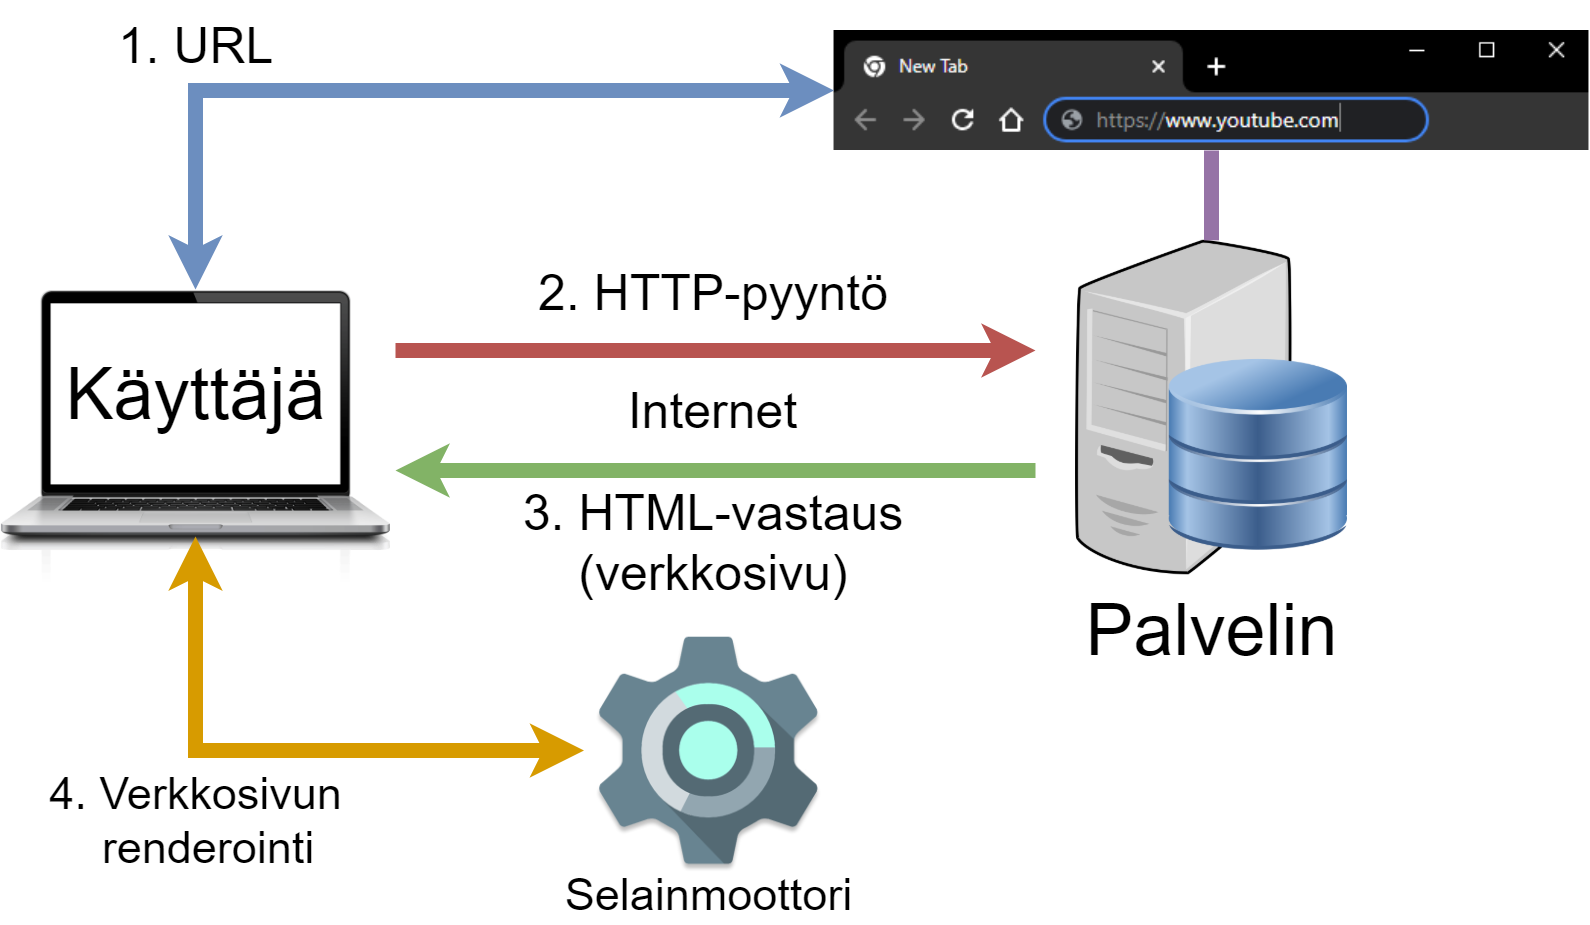
\includegraphics[height=8cm]{./img/browser.png}
  \caption{Yksinkertainen malli selaimen käyttöprosessista \label{kuva1}}
\end{figure}

\noindent Vaikka alkujaan internetin selaamiseen olikin olemassa vain muutamia selaimia, on niitä nykyään lukuisia erilaisia ja selaimia on tietokoneiden lisäksi useille eri laitteille, kuten älypuhelimet tablettitietokoneet, pelikonsolit ja älytelevisiot. Taulukossa 1 esitetyn tilaston mukaan tällä hetkellä viisi suosituinta tietokoneella käytettyä verkkoselainta ovat Google Chrome, Safari, Microsoft Edge, Mozilla Firefox ja Opera \cite{StatCounter}\cite{Similiarweb}. Tässä työssä keskitytään noihin viiteen selaimeen adaptiivisen videokuvan näkökulmasta. \\

\begin{table}[htb]
  \caption{Selainten markkinaosuus tietokonekäytössä helmikuussa 2022. \cite{StatCounter}\cite{Similiarweb} \label{taulukko1}}
  \centering
  \fbox{
    \begin{tabular}{l|l|l}
      Selain            & StatCounter & Similiarweb \\ \hline
      Google Chrome     & 64,91 \%    & 65,47 \% \\
      Safari            & 9,77 \%     & 10,04 \% \\
      Microsoft Edge    & 9,61 \%     & 11,34 \% \\
      Mozilla Firefox   & 9,47 \%     & 7,10 \% \\
      Opera             & 2,87 \%     & 1,94 \% \\
      Muut              & 3,37 \%     & 4,10 \%
    \end{tabular}
  }
\end{table}

\noindent Moderni verkkoselain koostuu useammasta komponentista, kuten käyttöliittymästä, selainmoottorista, muistista sekä JavaScript-tulkista. Kaikista keskeisin näistä komponenteista on selainmoottori eli selainydin. Selainmoottorin päätehtävänä on muuntaa HTML-tiedostot ja muut verkkosivun resurssit (kuten audio- ja videoresurssit) interaktiiviseksi visuaaliseksi esitykseksi käyttäjän laitteella. \\

\noindent Selainten mittavasta lukumäärästä huolimatta selainmoottoreita ei suinkaan ole yhtä montaa, ja suosituimmistakin selaimista peräti 3 käyttävät samaa selainydintä. Firefox käyttää Mozillan kehittämää Gecko-nimistä selainmoottoria, Safari käyttää Applen kehittämää WebKit-selainmoottoria ja Chrome, Edge sekä Opera käyttävät kaikki Chromium-projektille yhteistä Blink-selainmoottoria. \cite{Nield} Tämän työn kannalta merkittäviä selainmoottoreita ovat edellä mainitut Gecko, WebKit ja Blink, sillä viidessä suosituimmassa selaimessa on käytössä vain 3 eri selainmoottoria.

\noindent Verkkoselainten käyttöliittymä on selaimesta riippumatta usein hyvin samankaltainen. Yleensä selaimen käyttöliittymässä on ainakin seuraavat elementit:
\begin{itemize}
  \item[--] osoiterivi URL-osoitteiden syöttämiseen
  \item[--] eteenpäin ja takaisin navigoimista varten olevat painikkeet
  \item[--] kotipainike (joka vie käyttäjän asettamalle kotisivulle tai -sivuille)
  \item[--] päivitys- ja pysäytyspainike sivun resurssien päivittämiseen tai resurssien lataamisen pysäyttämiseen
  \item[--] kirjanmerkkien luomisen painike tai työkalut
  \item[--] hallintapainike, josta pääsee esimerkiksi selaimen asetuksiin
\end{itemize}
Vaikka moni muu ominaisuus verkkoselainten toiminnasta on standardien säätelemää, ei käyttöliittymän ominaisuuksista ole erillisiä standardeja. Silti yllä mainitut ja myös kuvassa 2 havaittavat ns. vakioelementit löytyvät lähes poikkeuksetta jokaisesta selaimesta tänä päivänä. Lisäksi selaimista löytyy usein jokin hakukone (esimerkiksi Google tai DuckDuckGo) integroituna osoiteriviin, välilehtijärjestelmä jonka avulla jokaista verkkosivua ei tarvitse avata omassa ikkunassaan sekä monia muita käytettävyyttä huomattavasti lisääviä ominaisuuksia.

\begin{figure}[htb]
  \centering
  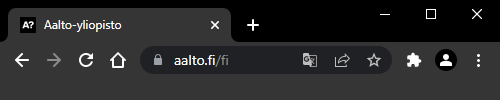
\includegraphics[height=3cm]{./img/browser-ui.png}
  \caption{Google Chrome -selaimen käyttöliittymä \label{kuva2}}
\end{figure}

\clearpage

% 3 Videokuva
\section{Videokuva}

Videokuvalla eli videolla tarkoitetaan yleensä teknologiaa, jolla elektronisista signaaleista muodostetaan liikkuvaa kuvaa. Video siis koostuu lähtökohtaisesti suuresta määrästä still-kuvia, jotka toistetaan nopeasti peräkkäin jolla simuloidaan liikettä. Videojärjestelmiä ja -teknologioita on nykyään hyvin monia erilaisia, ja niissä on useita eroavaisuuksia esimerkiksi näissä ominaisuuksissa:

\begin{itemize}
  \item[--] resoluutio eli kuvatarkkuus
  \item[--] kuvasuhde (kuvan leveys suhteessa korkeuteen)
  \item[--] virkistystaajuus eli montako kuvaa näytetään sekunnin aikana
  \item[--] väriominaisuudet
\end{itemize}

\noindent Videot olivat alun perin analogisia, joiden värijärjestelmiin ja koodausmenetelmiin kuuluivat muun muassa NTSC, PAL ja SECAM. Nykyään analogisia videoita käytetään kuitenkin enää harvoin, sillä internetin sekä usean digitaalisen tallennusvälineen ja järjestelmän käytön yleistymisen myötä myös digitaalisten videoiden määrä on kasvanut hurjasti. Lisäksi myös televisiolähetykset siirtyivät Suomessa kokonaan digitaaliseen formaattiin vuonna 2007 \cite{Digita}, mikä entisestään vähensi analogisen videon esiintyvyyttä. Tässä työssä käsitellään nimenomaan digitaalista videota etenkin suoratoistokäytössä. \\

\noindent Kuten videoiden toistamiseen ja katsomiseen on lukuisia erilaisia järjestelmiä, on digitaalisen videon formaatteja myös monia erilaisia. Videoformaateista puhutaan myös usein videosäiliöinä, joka on hyvin kuvaava, sillä videot usein sisältävät videosignaalin lisäksi myös ääntä. Taulukossa 2 on listattuna tämän hetken oleellisimpia digitaalisia videoformaatteja, sekä hieman avattu niiden pääsääntöisiä käyttökohteita. Kuten taulukossakin on mainittu, MP4 ja WebM ovat verkkokäyttöön parhaiten soveltuvat ja tästä johtuen suosituimmat formaatit. \\

\begin{table}[htb]
  \caption{Suosittuja videoformaatteja ja niiden käyttökohteita. \cite{Can I Use}\cite{Maayan}\cite{Adobe} \label{taulukko2}}
  \centering
  \fbox{
    \begin{tabular}{l|l|l}
      Videoformaatti  & Käyttö                      & Huomioita \\ \hline
      MP4             & Verkkosisältö, suoratoisto  & Selkeästi suosituin ja \\
                      &                             & käytetyin formaatti \\
      WebM            & Verkkosisältö, suoratoisto  & Monipuolinen, huono tuki \\
                      &                             & Applen alustoilla \\
      AVI             & TV ja päätiedostot          & Monipuolinen ja usein laadukas \\
                      &                             & formaatti, suuret tiedostokoot \\
      MOV             & Elokuvat ja TV              & Riippuvainen QuickTime- \\
                      &                             & ympäristöstä \\
      WMV             & Windows, suoratoisto        & Suhteellisen rajoittunut \\
                      &                             & Windows-ympäristöön \\
      Matroska        & Elokuvat ja TV              & AVI:n kaltainen \\
    \end{tabular}
  }
\end{table}

\noindent Syy MP4- ja WebM-formaattien suosioon löytyy niiden videodatan pakkaamiseen käytetyistä koodekeista. Yksi täysteräväpiirtovideon (1920x1080) kuva täydellä värillä (4 tavua per pikseli) on kooltaan 8 294 400 tavua. Tyypillisellä virkistystaajuudella (30 kuvaa sekunnissa) yksi sekunti täysteräväpiirtovideota vie siis 248 832 000 tavua tilaa eli noin 249 megatavua, yksi minuutti videota puolestaan noin 14,93 gigatavua ja yksi tunti videota olisi noin 895,8 gigatavua. Suhteutettaessa  internetyhteyden siirtonopeuksiin, olisi tällaisen pakkaamattoman videon suoratoisto siis todella vaativaa, sillä pelkän videoraidan siirto vaatisi 249 MB/s:n siirtonopeutta. \\

\noindent Jotta täysteräväpiirtovideon siirtäminen verkkoyhteyden avulla olisi realistista, tarvitsee videota pakata pienemmäksi. Videokoodekit ovat tässä avainasemassa. Koodekki on tässä yhteydessä ohjelmisto, jolla digitaalinen video voidaan pakata tietyn videokoodausformaatin mukaiseksi sekä purkaa kyseessä olevasta formaatista toistettavaksi signaaliksi \cite{Codec}. \\

\noindent Koodekista ja yhteensopivasta videokoodausformaatista käytetään usein samaa nimeä, jonka takia puhekielessä formaatin sijasta saatetaan helposti puhua koodekista. Tämän hetken yleisimpiin koodekkeihin sekä formaatteihin kuuluu muun muassa AV1, H.264/AVC, H.265/HEVC ja VP9 \cite{Codec guide}. Taulukosta 3 nähdään kootusti edellä mainittujen koodekkien tukemat säiliöformaatit. Taulukosta on havaittavissa hyvin nopeasti syy MP4-säiliön suosioon, sillä siihen voi sisällyttää kaikkia edellä mainittujen formaattien mukaista videota. Koodekeista H.264/AVC on vanhin ja heikoimmalla pakkaussuhteella varustettu, mutta myös yleisin ja tuetuin johtuen sen iästä. Uudemmat koodekit (etenkin AV1 ja H.265/AVC) taas omaavat selkeästi paremman pakkaussuhteen, mutta ovat vaihtelevammin tuettuna. Esimerkiksi YouTubessa videoita on tarjolla sekalaisilla koodekeilla koodattuna, joista etenkin uudemmat videot saattavat olla koodattu esimerkiksi AV1:llä tai H.265/HEVC:llä.

\begin{table}[htb]
  \caption{Suosittuja videokoodekkeja ja niiden säiliöitä. \cite{Codec guide} \label{taulukko3}}
  \centering
  \fbox{
    \begin{tabular}{l|l|l}
      Koodekki    & Koko nimi                     & Säiliötuki \\ \hline
      AV1         & AOMedia Video 1               & MP4, WebM \\
      H.264/AVC   & Advanced Video Coding	        & MP4, 3GP \\
      H.265/HEVC  & High Efficiency Video Coding  & MP4 \\
      VP9         & Video Processor 9             & MP4, WebM, Ogg \\
    \end{tabular}
  }
\end{table}

\subsection*{MP4}

MP4 eli MPEG-4 Part 14 on digitaalinen multimediasäiliöformaatti, jota käytetään lähtökohtaisesti videon ja äänen säilömiseen, mutta se voi sisältää näiden lisäksi myös erilaista dataa, kuten tekstitystä tai still-kuvia. MP4:n suosio verkkokäytössä johtuu pitkälti sen pienestä tiedostokoosta ja laajasta koodekkituesta. MP4 tukee esimerkiksi kaikkia taulukossa 3 mainittuja suosituimpia koodekkeja. MP4:ää käytetään formaattina etenkin koodekkien H.264 ja H.265 sekä myös AV1:n kanssa (tästä esimerkki kuvassa 3). \cite{Codecs}

\subsection*{WebM}

WebM on avoin ja rojaltivapaa audiovisuaalinen multimediasäiliöformaatti, joka suunniteltiin varta vasten korkealaatuiseksi avoimeksi standardiksi verkkokäyttöön. \cite{WebM} Ero WebM:n ja MP4:n välillä näkyy eniten ideologiaerona, sillä WebM tukee ainoastaan ilmaisia video- ja audiokoodekkeja. Tuettuihin koodekkeihin kuuluvat ensisijaisesti WebM-projektin itsensä kehittämät videokoodekit VP8 ja VP9 sekä Xiph Foundationin kehittämät audiokoodekit Vorbis ja Opus. WebM tukee myös AV1:tä, mutta AV1:n käyttö WebM-säiliössä on harvinaisempaa, kuin MP4-säiliössä (kuten kuvassa 3 näkyy). \cite{WebM FAQ}

\begin{figure}[htb]
  \centering
  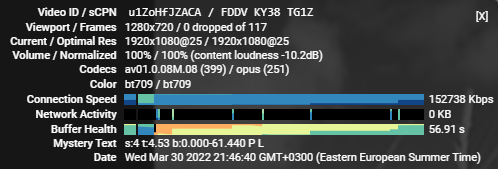
\includegraphics[height=4cm]{./img/youtube.png}
  \caption{Esimerkki YouTuben MP4-muotoisen videon teknisistä tiedoista. Videon koodekki on AV1 ja audion Opus. Videon formaatti selviää tutkimalla kehittäjä-näkymän verkko-osuutta. \label{kuva3}}
\end{figure}

\clearpage


% 4 Suoratoisto
\section{Suoratoisto}

Suoratoistolla, josta usein käytetään puhekielessä termiä striimaus, tarkoitetaan tiedonsiirtotapaa, jossa toistettava mediatiedosto siirretään kohteeseen jatkuvana tietovirtana siten, että tiedostoa voidaan prosessoida vastaanottavalla päätelaitteella jo ennen kuin koko tiedosto on lähetetty \cite{Britannica}. Esimerkiksi videota suoratoistettaessa videotiedostoa siis ladataan samanaikaisesti, kun sitä jo toistetaan päätelaitteella. Suoratoiston tarkoitus teknologiana on mahdollistaa median toistaminen nopeammin ja helpommin kuin perinteisellä tavalla, jossa koko tiedosto ladataan ensin käytettävälle laitteelle, jonka jälkeen sen voi vasta toistaa. Toistamisen nopeutus on huomattava, sillä huolimatta nykyaikaisten internet-yhteyksien nopeudesta, on esimerkiksi elokuvan lataaminen ja katsominen huomattavan hidas ja epämieluisa prosessi ilman suoratoistoteknologioita. Suoratoistoa käytetään usein esimerkiksi video- ja audiomedian siirtämiseen ja toistamiseen suoratoistopalveluiden, kuten Youtuben, Netflixin ja Spotifyn, toimesta. Suoratoistoteknologioiden käyttö ei kuitenkaan rajoitu vain video- ja äänimedian siirtämiseen ja toistamiseen, vaan sitä hyödynnetään myös muun muassa reaaliaikaiseen suoratoistoon. Teknologiat, kuten videopuhelut ja muu reaaliaikainen suoratoisto eli livestriimaus, sekä jopa pelien etäpelaaminen esimerkiksi Google Stadia -alustalla, \cite{Stadia} ovat esimerkkejä reaaliaikaisen suoratoiston käyttökohteista. Tässä työssä keskitytään erityisesti videoiden suoratoistoon sekä siihen liittyviin teknologioihin.

\subsection*{Adaptiivinen suoratoisto}

\noindent Siinä missä suoratoiston tarkoituksena on mahdollistaa median toistaminen nopeammin ja helpommin kuin koko tiedoston ensin lataamalla, on adaptiivisen suoratoiston tarkoituksena vielä tämän lisäksi taata käyttäjälle täysin katkoton median toistokokemus. Adaptiivisessa suoratoistossa eli adaptiivisen bittinopeuden suoratoistossa toistettava media on transkoodattu eri bittinopeuden mukaisiin ja eri laatuisiin toistettaviin muotoihin. Kuten kuvassa 4 on havainnollistettu, laadukkaampaa videota eli korkeammalla bittinopeudella olevaa varianttia toistetaan, kun käytössä on enemmän kaistanleveyttä. Käytettävän kaistanleveyden laskiessa toistettavan videon laatua lasketaan myös tarpeen mukaan ja toistettavaksi valitaan matalamman bittinopeuden variantti. \\

\begin{figure}[htb]
  \centering
  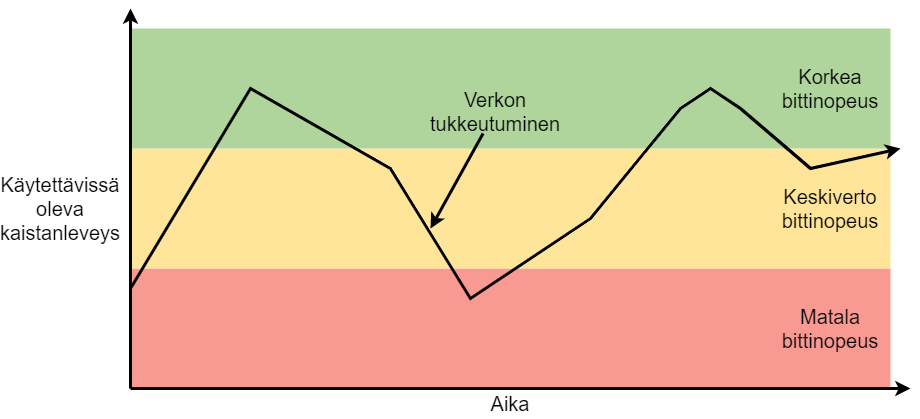
\includegraphics[height=6.5cm]{./img/abr-bandwidth.png}
  \caption{Adaptiivisen suoratoiston toiminnan mallinnus kaistanleveyden ja tukkeutumisen avulla \label{kuva4}}
\end{figure}

\noindent Tarkemmin kuvattuna adaptiivinen suoratoisto on siis metodi suoratoistaa videota, missä toistettava video on transkoodattu useille eri bittinopeuksille. Tärkeimmät adaptiivisen suoratoiston teknologiat on toteutettu HTTP:n pohjalle. Jokainen eri bittinopeuden virroista on lisäksi segmentoitu pieniin, usean sekunnin kestoisiin segmentteihin. Yhden segmentin kesto vaihtelee käytettävän toteutuksen mukaan, mutta segmentin pituus on usein kahden ja kymmenen sekuntin väliltä \cite{Segment}. Segmentit nimetään ja jaotellaan yksilöivästi, jonka jälkeen niistä koostetaan oikean järjestyksen mukainen soittolista. Tämä kyseinen soittolista rakentuu yleensä laadun mukaan lohkoihin jaotelluista numeroiduista videosegmenteistä ja audiosegmenteistä (riippuu toteutuksesta). Yleisesti käytössä on kahta tapaa: limitetty (engl. multiplexed) ja epälimitetty (engl. non-multiplexed). Limitetyssä toteutuksessa video- ja audiosegmentit ovat limittäin sijoitettu samalle tietovirralle ja ne ladataan peräkkäin vuorotellen samasta tietovirrasta. Limittämättömässä toteutuksessa käytössä on kaksi tietovirtaa: yksi videosegmenteille ja toinen audiosegmenteille. Tiedostoa, joka kertoo päätelaitteelle tämän kyseisen soittolistan sisällön ja tiedostojen peräkkäisen järjestyksen sekä muut videon toistamiseen tarvittavat tiedot, kutsutaan manifestiksi tai manifestitiedostoksi. \cite{Ottverse} \\

\begin{figure}[htb]
  \centering
  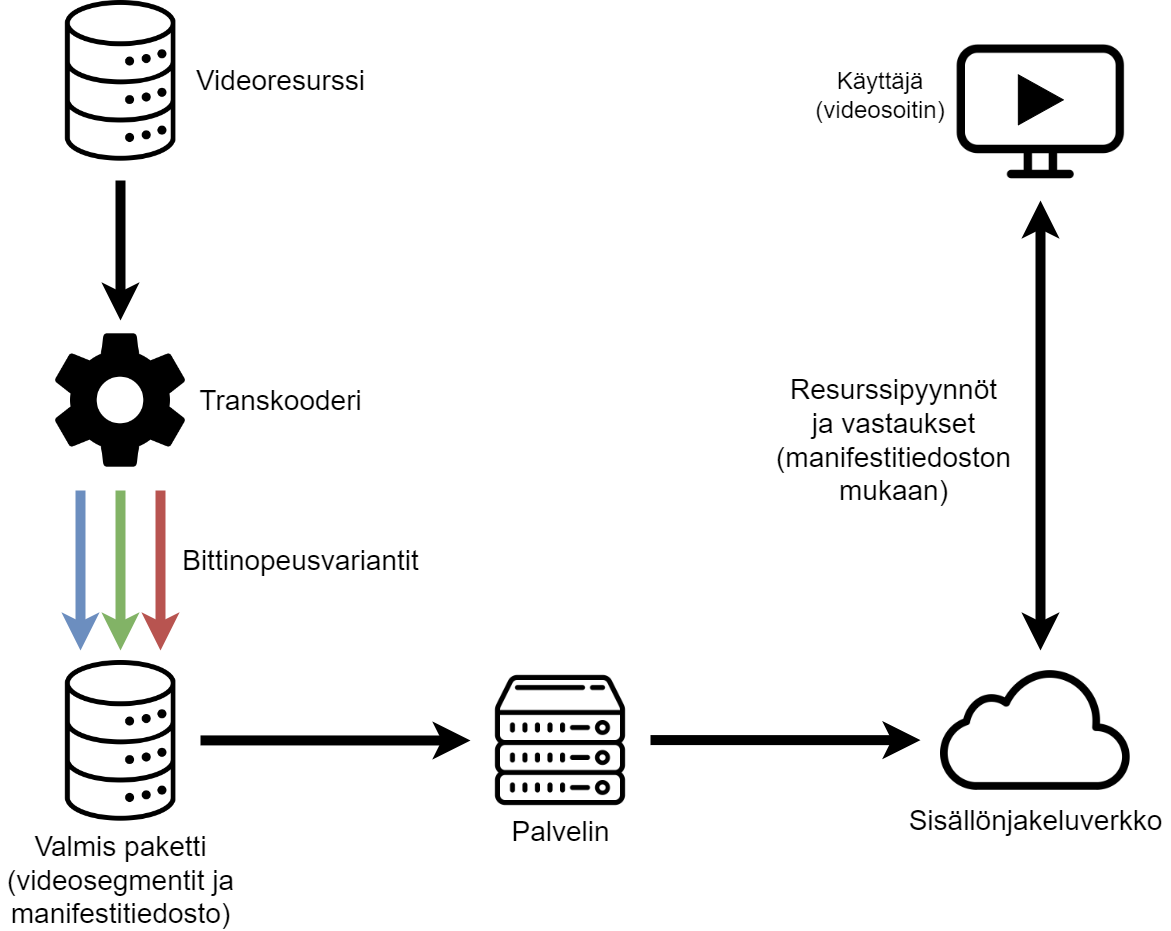
\includegraphics[height=11cm]{./img/abr-streaming.png}
  \caption{HTTP-perusteisen adaptiivisen suoratoiston toimintaperiaatteen visualisointi \label{kuva5}}
\end{figure}

\noindent Havainnollistava kaavio HTTP-perusteisen adaptiivisen suoratoistoteknologian, kuten DASH ja HLS (joista kerrotaan tarkemmin seuraavissa kappaleissa), käytöstä ja toiminnasta on esitetty kuvassa 5. Kun käyttäjä alkaa katsomaan videota verkkoselaimellaan (esimerkiksi YouTuben kautta), verkkoselain lataa ensimmäisenä videota koskevan manifestitiedoston. Tämän jälkeen verkkoselain selvittää manifestitiedostosta, mitä resursseja sen pitää ladata videon toistamiseksi. Selain tekee resurssipyyntöjä sisällönjakeluverkolle, jossa mediaresurssit sijaitsevat valmiina ladattavaksi, manifestitiedoston mukaisesti, jonka jälkeen kyseiset resurssit eli video- ja audiosegmentit ladataan sisällönjakeluverkosta käyttäjän laitteelle. Kun tarvittavat resurssit eli ensimmäinen tai ensimmäiset videosegmentit on ladattu käyttäjän laitteelle, verkkoselaimen videosoitin alkaa toistamaan videota. Jotta videon katselu ei olisi pätkivää, sisällönjakeluverkosta ladataan usein kerralla useampi segmentti varastoon puskuriksi, jos se on verkon käytettävissä olevan kaistanleveyden puitteissa mahdollista. Puskuriksi ladattavien segmenttien määrä vaihtelee toteutuksesta ja saatavilla olevasta kaistanleveydestä: mitä nopeampi yhteys ja enemmän kaistanleveyttä, sitä enemmän videosegmenttejä ehditään lataamaan puskuriin. Ladattavien videosegmenttien laatu valitaan yleensä aina edellisten segmenttien lataamisen jälkeen. Ohjelmisto tarkistaa saatavilla olevan kaistanleveyden, jonka mukaan valitaan kaistanleveystikkaasta, josta on esimerkki taulukossa 4, sopivan laatuinen videosegmentti tai -segmentit ladattavaksi. \cite{Ottverse} \\

\begin{table}[htb]
  \caption{Esimerkki siitä, miltä Dynamic Adaptive Streaming over HTTP:n kaistanleveystikas voisi näyttää. \cite{Bitrate ladder} \label{taulukko4}}
  \centering
  \fbox{
    \begin{tabular}{l|l}
      Kaistanleveys & Laatu \\ \hline
      5,0 Mb/s      & 1080p \\
      4,0 Mb/s      & 720p  \\
      3,2 Mb/s      & 640p  \\
      2.0 Mb/s      & 480p  \\
      1.0 Mb/s      & 270p  \\
    \end{tabular}
  }
\end{table}

\noindent HTTP-pohjaisia adaptiivisen suoratoiston teknologioita on useampia, joista kaksi tämän hetken merkittävintä ovat Dynamic Adaptive Streaming over HTTP sekä HTTP Live Streaming. Näitä kahta teknologiaa hyödyntävät useimmat suoratoisto- ja videopalvelut, kuten YouTube, Netflix, Disney+ ja Amazon Prime. Syynä HTTP-pohjaisen adaptiivisen suoratoistoteknologian suosioon on videoiden jakamisen helppoudessa. Koska sekä DASH että HLS perustuvat HTTP:hen, ne voivat kulkea minkä tahansa tavallisen palomuurin tai välityspalvelimen läpi, jotka sallivat tavanomaisen HTTP-liikenteen, joka ei ole mahdollista esimerkiksi UDP:hen perustuvassa RTP:ssä (Real-time Transport Protocol). Tämän takia DASH:in ja HLS:n hyödyntämiä viedoresursseja voidaan jakaa HTTP-pohjaisilla, laajasti tavoitettavissa olevilla sisällönjakeluverkoilla, jotka helpottavat videoresurssien saatavuutta entisestään. \\

\subsection*{DASH}

Dynamic Adaptive Streaming over HTTP, joka tunnetaan myös nimillä DASH ja MPEG-DASH, on ensimmäinen standardoitu HTTP-pohjainen adaptiivinen suoratoistoteknologia. DASH sai alkunsa, kun Moving Picture Experts Group (MPEG) teki CFP:n HTTP-pohjaisesta suoratoistostandardista vuonna 2009, jonka jälkeen sen kehitystyö alkoi vuonna 2010, johon osallistui useita alan yrityksiä ja organisaatioita. Alkuperäinen DASH-standardi julkaistiin huhtikuussa 2012, jonka jälkeen se on uusittu vuosina 2019 ja 2022. Teknologian osalta DASH toimii Media Source Extensioneiden (MSE) avulla, jotka mahdollistavat moderneissa selaimissa JavaScriptin lähettää tavuvirtoja selaimen mediakoodekkeihin ja sitä kautta esittää videota suoraan HTML5-teknologioilla. DASH on laajalti tuettu pitkälti kaikissa muissa selaimissa, paitsi Safarissa \cite{Lambdatest}.

\subsection*{HLS}

HTTP Live Streaming, josta käytetään usein lyhennettä HLS, on Applen kehittämä DASHia vastaava HTTP:hen perustuva adaptiivinen suoratoistoteknologia. HLS julkaistiin vuonna 2009 ja on julkaisunsa jälkeen ollut hyvin laajasti tuettuna erilaisissa mediasoittimissa, verkkoselaimissa ja mobiililaitteissa. Esimerkiksi vuonna 2018 HLS oli yhä DASH:tä suositumpi alan kehittäjien keskuudessa \cite{Bitmovin1}. Teknologian osalta HLS voi selaimesta riippuen toimia joko natiivisti tai MSE:n avulla, kuten DASH. HLS on tuettu kaikissa moderneissa selaimissa. \cite{Spiceworks}

\clearpage


% 5 Vertailu
\section{Vertailu}

Pintapuolisesti tarkasteltuna adaptiivisen videokuvan katselu ei eroa juuri mitenkään eri selaimilla. Isoimmat erot käyttäjälle näkyvät selainten erilaisten käyttöliittymien ja muiden ominaisuuksien muodossa. Kuitenkin eroja esimerkiksi videon latausnopeudessa sekä laadussa voi ilmetä, johtuen käytetystä videon eri koodekista tai formaatista, joiden tuki vaihtelee selaimittain. Tästä selkeimpänä esimerkkinä lienee AV1, jota Safari ei tue lainkaan tällä hetkellä, kun taas muut selaimet tukevat AV1-koodattuja videoita. AV1:n erinomainen pakkaussuhde sekä korkea laatu tiedostokokoon nähden voivat näkyä erona nopeudessa ja laadussa käyttäjille. \\

\noindent Suurimmat erot videoiden adaptiivisessa suoratoistossa verkkoselaimilla piilee ulkokuoren alla käytettävissä teknologioissa. Eri videopalvelut suosivat joko DASH:ä tai HLS:ää ja täten samaa selainta käyttäessä eri videopalveluiden videot voivat olla toimitettu eri menetelmällä. Vaikka videopalvelulla olisi suuri preferenssi DASH:ä kohtaan, on videopalvelun kuitenkin pakko tarjota videoita myös HLS:llä, sillä muuten kaikki Safari-käyttäjät jäisivät ilman videoita. Ottaen Safari-käyttäjien suuren määrän huomioon, kyseessä on tarpeeksi iso osuus videoiden katsojakunnasta, ettei videopalvelut voi jättää heitä huomiotta. Toisin sanoen Apple pakottaa videopalvelut tarjoamaan videonsa myös HLS:n avulla, sillä Safariin ei ole lisätty DASH-tukea. Esimerkiksi YouTube on ilmoittanut käyttävänsä DASH:ä aina kun mahdollista \cite{Bitmovin2}. Myös Netflix on ilmoittanut tähtäävänsä tarjoamaan videosisältönsä lähtökohtaisesti DASH:llä ja mieluiten AV1-koodattuna \cite{Netflix}. Kuitenkin molemmat näistä videopalveluista tarjoaa sisältöä myös HLS:llä, aivan kuten muutkin videopalvelut. \\

\noindent Eroja selainten välillä on myös käytetyissä koodekeissa. Siinä missä Safari ei tue AV1:tä, eivät Chrome, Firefox, Opera ja Edge tue H.265/HEVC:tä, toisin kuin Safari. Safari on siis ainoa, joka tukee lisenssimaksullista HEVC:tä korkeampana laatuvaihtoehtona H.264/AVC:n sijasta, kun taas muilla selaimilla käytössä on koodekit H.264/AVC, VP9 ja AV1, joista valtaosa on lisenssimaksuttomia. Muilla selaimilla on siis huomattavasti enemmän vaihtoehtoja koodekkien suhteen ja preferoivat usein monien vidoepalveluiden lailla ilmaisia vaihtoehtoja. \\

\noindent Havaittavissa on siis kahta koulukuntaa: Apple ja muut alan toimijat. Apple on käytännössä pakottanut teknologiavalintoja siirtoprotokollan ja koodekkien muodossa ja täten pakottanut videopalvelut tarjoamaan sisältöä sen sanelemilla ehdoilla, sillä tarpeeksi iso osa internetin videopalveluiden käyttäjistä käyttää Safaria selaimenaan.

\clearpage


% 6 Yhteenveto
\section{Yhteenveto}

Kaiken kaikkiaan modernit työssä tarkastellut verkkoselaimet ovat hyvin samanlaisia, ja niissä on monipuolisesti erilaisia ominaisuuksia. Selainmoottoreita on käytössä vain 3 (WebKit, Gecko ja Blink), joista Blink on selkeästi käytetyin. \\

\noindent Nykyään videoformaatteja on olemassa hyvin monenlaisia, mutta niistä erityisesti MP4 ja WebM ovat laajassa käytössä internetin suoratoistovideopalveluissa. Sekä MP4 että WebM omaavat todella hyvän pakkaussuhteen, eli niihin voidaan säilöä laadukasta videosisältöä pitämällä tiedostokoko kuitenkin minimissä. Molemmpiin formaatteihin voidaan säilöä useammalla eri koodekilla koodattua video- ja audiodataa. MP4 on näistä kahdesta monipuolisempi formaatti, sillä WebM lähtökohtaisesti tukee ainoastaan ilmaisia video- ja audiokoodekkeja. \\

\noindent Tämän hetken käytetyimmät videokoodekit ovat H.264/AVC, VP9, H.265/HEVC ja AV1. Edellä mainitusta neljästä koodekista AVC ja HEVC ovat lisenssimaksullisia, kun taas VP9 ja AV1 ovat ilmaisia. Edellä mainituista H.264/AVC ja VP9 on tuettu kaikissa selaimissa. H.265/HEVC on tuettu vain Safarissa, kun taas muut selaimet tukevat sen sijasta AV1:tä paremman laadun koodekkina. \\

\noindent Lähes kaikki adaptiivisen suoratoiston videot toimitetaan HTTP:hen perustuvilla teknologioilla. Näistä kaksi tärkeintä toteutusta ovat DASH ja HLS, joilla lähes kaikki adaptiivinen suoratoisto tuntuu olevan toteutettu internetissä. DASH ja HLS ovat toimintaperiaatteeltaan lähes identtiset, sillä niiden suurimmat erot löytyvät lähinnä manifestitiedostosta. Molemmissa video on jaettu pieniin, muutaman sekunnin mittaisiin segmentteihin ja kaikki segmentit on saatavissa myös eri laatuisina. Ladattava laatu valitaan aina käytettävissä olevan kaistanleveyden mukaan, jolloin toisto on katkotonta. \\

\noindent Tutkimuksessa havaitaan, että kaikki käsitellyt selaimet ovat varsin toimivia käyttötarkoitukseensa ja täten selainvalinnalla ei ole paljoa merkitystä yleisesti ottaen adaptiivisen suoratoistovideon katselussa. Tutkimus kuitenkin antaa osviittaa, että paras selainvalinta olisi todennäköisesti Google Chrome, sillä se hyödyntää ja tukee lähtökohtaisesti uusimpia teknologioita ja omaa laajimman käyttäjäkunnan. Tutkimus myös osoittaa, että käsitellyistä selaimista Safari olisi huonoin, sillä se tukee vähemmän protokollia ja teknologioita, kuin esimerkiksi kilpailijansa.

\clearpage


% Viitteet
\thesisbibliography
\begin{thebibliography}{99}

  \bibitem{Hauben}
    M.\ Hauben, R.\ Hauben.
    \textit{Behind the Net: The Untold History of the ARPANET and Computer Science (Chapter 7).}
    Verkkodokumentti.
    Viitattu: 27.2.2022.
    Saatavissa: \url{doi:10.5210/fm.v3i8.612}.

  \bibitem{ITU}
    \textit{Measuring digital development: Facts and figures 2021.}
    ISBN 978-92-61-35401-5.
    2021.
    Telecommunication Development Bureau, International Telecommunication Union (ITU).
    Viitattu: 27.2.2022.
    Saatavissa: \url{https://www.itu.int/itu-d/reports/statistics/facts-figures-2021/}.

  \bibitem{SVT}
    \textit{Suomen virallinen tilasto (SVT): Väestön tieto- ja viestintätekniikan käyttö.}
    ISSN 2341-8699 [verkkojulkaisu].
    2018.
    Helsinki: Tilastokeskus.
    Viitattu: 27.2.2022.
    Saatavissa: \url{http://www.stat.fi/til/sutivi/2018/sutivi_2018_2018-12-04_tie_001_fi.html}.

  \bibitem{WorldWideWeb}
    T.\ Berners-Lee.
    \textit{The WorldWideWeb browser.}
    Verkkodokumentti.
    Viitattu: 15.3.2022.
    Saatavissa: \url{https://www.w3.org/People/Berners-Lee/WorldWideWeb.html}.

  \bibitem{URL}
    \textit{What is a URL?.}
    Verkkodokumentti.
    Viitattu: 15.3.2022.
    Saatavissa: \url{https://developer.mozilla.org/en-US/docs/Learn/Common_questions/What_is_a_URL}.

  \bibitem{StatCounter}
    \textit{Desktop Browser Market Share Worldwide Feb 2022.}
    StatCounter Globalstats.
    Viitattu: 15.3.2022.
    Saatavissa: \url{https://gs.statcounter.com/browser-market-share/desktop/worldwide/#monthly-202202-202202-bar}.

  \bibitem{Similiarweb}
    \textit{Top Desktop Browsers Market Share in February 2022.}
    Similiarweb.
    Viitattu: 29.3.2022.
    Saatavissa: \url{https://www.similarweb.com/browsers/worldwide/desktop/}.

  \bibitem{Nield}
    D.\ Nield.
    \textit{Which Browser Engine Powers Your Web Browsing — And Why Does It Matter?.}
    12.4.2019.
    Verkkodokumentti.
    Viitattu: 16.3.2022.
    Saatavissa: \url{https://gizmodo.com/which-browser-engine-powers-your-web-browsing-and-why-d-1833935288}.

  \bibitem{Digita}
    \textit{Digitaalisen television kehitysvaiheet Suomessa.}
    Verkkodokumentti.
    Viitattu: 24.3.2022.
    Saatavissa: \url{https://www.digita.fi/antennitv/vapaat-kanavat-ja-vastaanotto/hyodyllista-tietoa-tvsta/kehitysvaiheet/}.

  \bibitem{Codec}
    \textit{Video Codec.}
    Verkkodokumentti.
    Viitattu: 30.3.2022.
    Saatavissa: \url{https://www.pcmag.com/encyclopedia/term/video-codec}.

  \bibitem{Can I Use}
    \textit{Browser support tables for modern web technologies — Can I use video format?.}
    Verkkodokumentti.
    Viitattu: 24.3.2022.
    Saatavissa: \url{https://caniuse.com/?search=video%20format}.

  \bibitem{Maayan}
    G.\ Maayan.
    \textit{8 Best Video File Formats for 2020.}
    Verkkodokumentti.
    Viitattu: 24.3.2022.
    Saatavissa: \url{https://www.computer.org/publications/tech-news/trends/8-best-video-file-formats-for-2020}.

  \bibitem{Adobe}
    \textit{Choosing the right video format.}
    Verkkodokumentti.
    Viitattu: 24.3.2022.
    Saatavissa: \url{https://www.adobe.com/uk/creativecloud/video/discover/best-video-format.html}

  \bibitem{Codec guide}
    \textit{Web video codec guide.}
    Verkkodokumentti.
    Viitattu: 30.3.2022.
    Saatavissa: \url{https://developer.mozilla.org/en-US/docs/Web/Media/Formats/Video_codecs}.

  \bibitem{Codecs}
    \textit{Codecs.}
    Verkkodokumentti.
    Viitattu 8.9.2022.
    Saatavissa: \url{http://mp4ra.org/#/codecs}.

  \bibitem{WebM}
    \textit{About WebM.}
    Verkkodokumentti.
    Viitattu: 30.3.2022.
    Saatavissa: \url{https://www.webmproject.org/about/}.

  \bibitem{WebM FAQ}
    \textit{Frequently Asked Questions - WebM}
    Verkkodokumentti.
    Viitattu: 8.9.2022.
    Saatavissa: \url{https://www.webmproject.org/about/faq/}.

  \bibitem{Britannica}
    \textit{streaming | Definition, Meaning and Facts | Brotannica.}
    Verkkodokumentti.
    Viitattu: 17.5.2022.
    Saatavissa: \url{https://www.britannica.com/topic/streaming-data-transmission}.

  \bibitem{Stadia}
    \textit{Stadia - Yksi paikka kaikille pelitavoille.}
    Verkkodokumentti.
    Viitattu: 17.5.2022.
    Saatavissa: \url{https://stadia.google.com/}.

  \bibitem{Ottverse}
    \textit{What is MPEG-DASH Video Streaming Protocol? How Does MPEG-DASH Work?.}
    Verkkodokumentti.
    Viitattu: 8.9.2022.
    Saatavissa: \url{https://ottverse.com/mpeg-dash-video-streaming-the-complete-guide/}

  \bibitem{Segment}
    \textit{Optimal Adaptive Streaming Formats MPEG-DASH & HLS Segment Length.}
    Verkkodokumentti.
    Viitattu: 1.6.2022.
    Saatavissa: \url{https://bitmovin.com/mpeg-dash-hls-segment-length/}.

  \bibitem{Bitrate ladder}
    \textit{MPEG-DASH (Dynamic Adaptive Streaming over HTTP) Explained.}
    Verkkodokumentti.
    Viitattu 1.9.2022.
    Saatavissa: \url{https://corp.kaltura.com/blog/mpeg-dash/}.

  \bibitem{Lambdatest}
    \textit{Browser Compatibility Of Dynamic Adaptive Streaming Over HTTP (MPEG-DASH) On Safari 7.1.}
    Verkkodokumentti.
    Viitattu 7.9.2022.
    Saatavissa: \url{https://www.lambdatest.com/web-technologies/mpeg-dash-support-on-safari-7.1}.

  \bibitem{Spiceworks}
    \textit{MPEG-DASH vs HLS: Which One Should You Use?.}
    Verkkodokumentti.
    Viitattu: 8.9.2022.
    Saatavissa: \url{https://www.spiceworks.com/tech/programming/guest-article/mpeg-dash-vs-hls-which-one-should-you-use/}

  \bibitem{Bitmovin1}
    \textit{Video Developer Report 2018.}
    Verkkodokumentti.
    Viitattu: 6.9.2022.
    Saatavissa: \url{https://go.bitmovin.com/hubfs/Bitmovin-Video-Developer-Report-2018.pdf}.

  \bibitem{Bitmovin2}
    \textit{Why YouTube & Netflix use MPEG-DASH in HTML5.}
    Verkkodokumentti.
    Viitattu: 7.9.2022.
    Saatavissa: \url{https://bitmovin.com/mpeg-dash-youtube-netflix-html5/}.

  \bibitem{Netflix}
    \textit{Netflix Now Streaming AV1 on Android.}
    Verkkodokumentti.
    Viitattu: 7.9.2022.
    Saatavissa: \url{https://netflixtechblog.com/netflix-now-streaming-av1-on-android-d5264a515202}

\end{thebibliography}

\end{document}
